\chapter{Parameter Inference}
\label{ch:fastinference}

In this chapter\footnote{%
This chapter is based on \citet{maystre2015fast}.},
we study the problem of inferring parameters of models derived from Luce's choice axiom.
We begin by showing that the maximum-likelihood estimate (MLE) can be expressed as the stationary distribution of a Markov chain.
This conveys insight into several recently proposed spectral inference algorithms.
We then take advantage of this perspective and formulate a new spectral algorithm that generalizes and improves upon prior work.
With a simple adaptation, this algorithm can be used iteratively, producing a sequence of estimates that converges to the MLE.
The MLE version runs faster than competing approaches on a benchmark of five datasets.

%%%%%%%%%%%%%%%%%%%%%%%%%%%%%%%%%%%%%%%%%%%%%%%%%%%%%%%%%%%%%%%%%%%%%%%%%
\section{Introduction}  %%%%%%%%%%%%%%%%%%%%%%%%%%%%%%%%%%%%%%%%%%%%%%%%%
\label{sec:introduction}

Consider the problem of estimating click probabilities for links between pages of a website, given a hyperlink graph and aggregate statistics on the number of times each page has been visited.
Naively, one might expect that the probability of clicking on a particular link should be roughly proportional to the traffic of the link's target.
%At first, one might expect that links pointing to high-traffic web pages must be more likely to be clicked.
However, this neglects important structural effects:
a page's traffic is influenced by
\begin{enuminline}
\item the number of incoming links,
\item the traffic at the pages that link to it, and
\item the traffic absorbed by competing links.
\end{enuminline}
In order to successfully infer click probabilities, it is therefore necessary to disentangle the \emph{preference} for a page (i.e., the intrinsic propensity of a user to click on a link pointing to it) from the page's \emph{visibility} (the exposure it gets from pages linking to it).
Building upon recent work by \citet{kumar2015inverting}, we present a statistical framework that tackles a general formulation of the problem:
given a network (representing possible transitions between nodes) and the marginal traffic at each node, recover the transition probabilities.
This problem is relevant to a number of scenarios (in social, information or transportation networks) where transition data is not available due to, e.g., privacy concerns or monitoring costs.

%Our starting point is a choice model, i.e., a model that explains and predicts outcomes of comparisons between two or more alternatives from a universe of $n$ items.
%In this context, a prominent paradigm (which dates back to \citet{thurstone1927method} and \citet{zermelo1928berechnung} almost a century ago) postulates that each item can be characterized by a latent \emph{strength} parameter, and that the (stochastic) comparison outcomes tend to favor items with greater strengths.
%The parameters can be learned from observed choices and used for predicting future comparisons.
%Models based on this paradigm have been successfully applied to problems ranging from ranking chess players based on game outcomes \citep{zermelo1928berechnung, elo1978rating} to understanding consumer behavior based on discrete choices \citep{mcfadden1973conditional}, and to discriminating among multiple classes based on the output of pairwise classifiers \citep{hastie1998classification}.
%Here, we assume that the comparisons are generated from a specific stochastic process on a network, reminiscent of the random-surfer model introduced by \citet{brin1998anatomy}.
%In our setting, every node in the network represents an item, and comparisons take place over the $n$ sets of alternatives induced by the neighborhoods of each node.
We begin by postulating the following model of traffic.
Users navigate from node to node along the edges of the network by making a choice between adjacent nodes at each step, reminiscent of the random-surfer model introduced by \citet{brin1998anatomy}.
Choices are assumed to be independent and generated according to Luce's model \citep{luce1959individual}: each node in the network is chararacterized by a latent \emph{strength} parameter, and (stochastic) choice outcomes tend to favor nodes with greater strengths.
In this model, estimating the transition probabilities amounts to estimating the strength parameters.
Unlike the setting in which choice models are traditionally studied \citep{train2009discrete, maystre2015fast, vojnovic2016parameter}, we do not observe distinct choices among well-identified sets of alternatives.
Instead, we only have access to aggregate, marginal statistics about the traffic at each node in the network.
In this setting, we make the following contributions.

\begin{enumerate}
\item We observe that marginal per-node traffic is a sufficient statistic for the strength parameters.
That is, the parameters can be inferred from marginal traffic data without any loss of information.

\item We show that if the parameters are endowed with a prior distribution, the inference problem becomes well-posed regardless of the network structure.
This is a crucial step in making the framework applicable to real-world datasets.

\item We show that model inference can scale to very large datasets.
We present an iterative EM-type inference algorithm that enables a remarkably efficient implementation---each iteration requires the computational equivalent of two iterations of PageRank.
\end{enumerate}

%To summarize our contributions from a machine-learning practitioner's perspective, we propose a scalable method that is able to learn transition probabilities in a network, given only the network's structure and the marginal traffic at each node.

We evaluate two aspects of our framework using real-world networks.
We begin by demonstrating that local preferences can indeed be inferred from global traffic: we investigate the accuracy of the transition probabilities recovered by our model on three datasets for which we have ground-truth transition data.
First, we consider two hyperlink graphs, representing the English Wikipedia (over two million nodes) and a Hungarian news portal (approximately \num{40000} nodes), respectively.
We model clickstream data as a sequence of independent choices over the links available at each page.
Given only the structure of the graph and the marginal traffic at every node, we estimate the number of transitions between nodes, and we find that our estimate matches ground-truth edge-level transitions accurately in both instances.
Second, we consider the network of New York City's bicycle-sharing service.
For a given ride, given a pick-up station, we model the drop-off station as a choice out of a set of locations.
Our model yields promising results, suggesting that our method can be useful beyond clickstream data.
Next, we test the scalability of the inference algorithm.
We show that the algorithm is able to process a snapshot of the WWW hyperlink graph containing over a hundred billion edges using a single machine.


\paragraph{Organization of the paper.}
In Section~\ref{sec:model}, we formalize the network choice model.
In Section~\ref{sec:relwork}, we briefly review related literature.
In Section~\ref{sec:theory}, we present salient statistical properties of the model and its maximum-likelihood estimator, and we propose a prior distribution that makes the inference problem well-posed.
In Section~\ref{sec:algorithm}, we describe an inference algorithm that enables an efficient implementation.
We evaluate the model and the inference algorithm in Section~\ref{sec:experiments}, before concluding in Section~\ref{sec:conclusion}.
In the appendices, we provide a more in-depth discussion of our model and algorithm, and we present proofs for all the theorems stated in the main text.

%%%%%%%%%%%%%%%%%%%%%%%%%%%%%%%%%%%%%%%%%%%%%%%%%%%%%%%%%%%%%%%%%%%%%%%%%
\section{Related Work}  %%%%%%%%%%%%%%%%%%%%%%%%%%%%%%%%%%%%%%%%%%%%%%%%%
\label{cr:sec:relwork}

A variant of the network choice model was recently introduced by \citet{kumar2015inverting}, in an article that lays much of the groundwork for this chapter.
Their generative model of traffic and the parametrization of transition probabilities based on Luce's axiom form the basis of our work.
\citeauthor{kumar2015inverting} define the \emph{steady-state inversion} problem as follows:
Given a graph $\mathcal{G}$ and a target stationary distribution, find transition probabilities that lead to the desired stationary distribution.
This problem formulation assumes that $\mathcal{G}$ satisfies restrictive structural properties (strong-connectedness, aperiodicity) and is valid only asymptotically, when the sequences of choices made by users are very long.
Our formulation is, in contrast, more general.
In particular, we eliminate any assumptions about the structure of $\mathcal{G}$ and cope with finite data in a principled way---in fact, our derivations are valid for choice sequences of any length.
One of our contributions is to explain the steady-state inversion problem in terms of (asymptotic) maximum-likelihood inference in the network choice model.
Furthermore, the statistical viewpoint that we develop also leads to
\begin{enuminline}
\item a robust regularization scheme, and
\item a simple and efficient EM-type inference algorithm.
\end{enuminline}
These important extensions make the model easier to apply to real-world data.

\paragraph{Luce's Choice Axiom}
The general problem of estimating parameters of models based on Luce's axiom has received considerable attention.
Several decades before Luce's seminal book \citep{luce1959individual}, \citet{zermelo1928berechnung} proposed a model and an algorithm that estimates the strengths of chess players based on pairwise comparison outcomes (his model would later be rediscovered by \citet{bradley1952rank}).
More recently, \citet{hunter2004mm} explained \citeauthor{zermelo1928berechnung}'s algorithm from the perspective of the minorization-maximization (MM) method.
This method is easily generalized to other models that are based on Luce's axiom, and it yields simple, provably convergent algorithms for maximum-likelihood (ML) or maximum-a-posteriori point estimates.
\citet{caron2012efficient} observe that these MM algorithms can be further recast as expectation-maximization (EM) algorithms by introducing suitable latent variables.
They use this observation to derive Gibbs samplers for a wide family of models.
We take advantage of this long line of work in Section~\ref{cr:sec:inference} when developing an inference algorithm for the network choice model.
In recent years, several authors have also analyzed the sample complexity of the ML estimate in Luce's choice model \citep{hajek2014minimax, vojnovic2016parameter} and investigated alternative spectral inference methods \citep{negahban2012iterative, azari2013generalized, maystre2015fast}.
Some of these results could be applied to our setting, but in general they require observing choices among well-identified sets of alternatives.
Finally, we note that models based on Luce's axiom have been successfully applied to problems ranging from ranking players based on game outcomes \citep{zermelo1928berechnung, elo1978rating} to understanding consumer behavior based on discrete choices \citep{mcfadden1973conditional}, and to discriminating among multiple classes based on the output of pairwise classifiers \citep{hastie1998classification}.

\paragraph{Network Analysis}
Understanding the preferences of users in networks is of significant interest in many domains.
For brevity, we focus on literature related to hyperlink graphs.
A method that has undoubtedly had a tremendous impact in this context is PageRank \citep{brin1998anatomy}.
PageRank computes a set of scores that are proportional to the amount of time a surfer, who clicks on links randomly and uniformly, spends at each node.
These scores are based only on the structure of the graph.
The network choice model presented in this chapter appears similar at first, but tackles a different problem.
In addition to the structure of the graph, it uses the traffic at each page, and computes a set of scores that reflect the (non-uniform) probability of clicking on each link.
Nevertheless, there are striking similarities in the implementation of the respective inference algorithms (see Section~\ref{cr:sec:experiments}).
The HOTness method proposed by \citet{tomlin2003new} is somewhat related, but tries to tackle a harder problem.
It attempts to estimate jointly the traffic and the probability of clicking on each link, by using a maximum-entropy approach.
At the other end of the spectrum, BrowseRank \citep{liu2008browserank} uses detailed data collected in users' browsers to improve on PageRank.
Our method uses only marginal traffic data that can be obtained without tracking users.
%In the context of mobility analysis, we mention that \citet{ashbrook2003using} and \citet{kafsi2015traveling}

%%%%%%%%%%%%%%%%%%%%%%%%%%%%%%%%
\section{Algorithms}
\label{fi:sec:algorithms}

We begin by expressing the MLE under the choice model as the stationary distribution of a Markov chain.
We then take advantage of this formulation to propose novel algorithms for model inference.
Although our derivation is made in the general choice model, we will also discuss implications for the special cases of pairwise data in Section~\ref{fi:sec:pairwise}, $K$-way ranking data in Section~\ref{fi:sec:partial}, and pairwise comparisons with ties in Section~\ref{fi:sec:ties}.

\subsection{MLE as a Stationary Distribution}

For each item $i \in [N]$, we define two sets of indices.
Let $\mathcal{W}_i \doteq \{ m : i \in \mathcal{A}_m, c_m = i \}$ and $\mathcal{L}_i \doteq \{ m : i \in \mathcal{A}_m, c_m \ne i \}$ be the indices of the observations where item $i$ wins over and loses against the alternatives, respectively.
We start from the log-likelihood $\ell(\bm{\gamma})$ in~\eqref{fi:eq:loglik};
the optimality condition $\nabla \ell = 0$ implies
\begin{align}
\left. \frac{\partial \ell(\bm{\gamma})}{\partial \gamma_i} \right\rvert_{\bm{\gamma} = \bm{\gamma}^\star}
    = \sum_{m \in W_i} \bigg[ \frac{1}{\gamma^\star_i} - \frac{1}{\sum_{j \in \mathcal{A}_m} \gamma^\star_j} \bigg]
      - \sum_{m \in \mathcal{L}_i} \frac{1}{\sum_{j \in \mathcal{A}_m} \gamma^\star_j} = 0 \quad \forall i \label{fi:eq:step1} \\
\iff  \sum_{j \ne i} \left[
    \sum_{m \in \mathcal{W}_i \cap \mathcal{L}_j} \frac{\gamma^\star_j}{\sum_{k \in \mathcal{A}_m} \gamma^\star_k}
    \;-\; \sum_{m \in \mathcal{W}_j \cap \mathcal{L}_i} \frac{\gamma^\star_i}{\sum_{k \in \mathcal{A}_m} \gamma^\star_k}
    \right] = 0 \quad \forall i. \label{fi:eq:mlbalance}
\end{align}
In order to go from \eqref{fi:eq:step1} to \eqref{fi:eq:mlbalance}, we multiply by $\gamma^\star_i$ and rearrange the terms.
To simplify the notation, let us further introduce the function
\begin{align*}
f(\mathcal{S}, \bm{\gamma}) \doteq \sum_{\mathcal{A} \in \mathcal{S}} \frac{1}{\sum_{i \in \mathcal{A}} \gamma_i},
\end{align*}
which takes observations $\mathcal{S} \subseteq \mathcal{D}$ and an instance of model parameters $\bm{\gamma}$, and returns a non-negative real number.
Let $\mathcal{D}_{i \succ j} \doteq \{ (c_m, \mathcal{A}_m) \in \mathcal{D} : m \in \mathcal{W}_i \cap \mathcal{L}_j \}$, i.e., the set of observations where $i$ wins over $j$.
Then \eqref{fi:eq:mlbalance} can be rewritten as
\begin{align}
\label{fi:eq:master}
\sum_{j \ne i} \gamma^\star_i \cdot f(\mathcal{D}_{j \succ i}, \bm{\gamma}^\star)
= \sum_{j \ne i} \gamma^\star_j \cdot f(\mathcal{D}_{i \succ j}, \bm{\gamma}^\star) \quad \forall i.
\end{align}
This formulation conveys a new viewpoint on the MLE.
It is easy to recognize the global balance equations \eqref{fi:eq:balance} of a Markov chain on $N$ states (representing the items), with transition rates $\lambda_{ji} = f(\mathcal{D}_{i \succ j}, \bm{\gamma}^\star)$ and stationary distribution $\bm{\gamma}^\star$.
These transition rates have an interesting interpretation: $f(\mathcal{D}_{i \succ j}, \bm{\gamma})$ is the count of how many times $i$ wins over $j$, weighted by the strength of the alternatives.
At this point, it is useful to observe that for any parameters $\bm{\gamma}$, $f(\mathcal{D}_{i \succ j}, \bm{\gamma}) > 0$ if and only if $(j,i) \in \mathcal{E}$.
Combined with the assumption that $\mathcal{G}$ is strongly connected, it follows that any $\bm{\gamma}$ parametrizes the transition rates of an ergodic (homogeneous) Markov chain.
The ergodicity of the inhomogeneous Markov chain, where the transition rates are constantly updated to reflect the current distribution over states, is shown by the following theorem.
\begin{theorem}
\label{fi:thm:convergence}
The Markov chain with inhomogeneous transition rates $\lambda_{ji} = f(\mathcal{D}_{i \succ j}, \bm{\gamma})$ converges to the maximum-likelihood estimate $\bm{\gamma}^\star$, for any initial distribution in the open probability simplex.
\end{theorem}

\begin{proof}[Proof]
Let $\bm{Q}(\bm{\gamma})$ be the infinitesimal generator matrix of the Markov chain $\bm{\gamma}(t)$.
The dynamics of the Markov chain are described by the differential equation
\begin{align}
\label{fi:eq:dynsys}
\frac{d \bm{\gamma}}{dt} = \bm{\gamma}^\Tr \bm{Q}(\bm{\gamma}).
\end{align}
By construction, the invariant distributions of the Markov chain coincide with the maximizers of the log-likelihood~\eqref{fi:eq:loglik}.
Hence, we know that $\bm{\gamma}^\star$ is the unique equilibrium point for~\eqref{fi:eq:dynsys}, i.e., satisfying $\bm{\gamma}^\Tr \bm{Q}(\bm{\gamma}) = \bm{0}$.
We will now show that this point is globally and asymptotically stable, i.e., $\bm{\gamma}(t) \to \bm{\gamma}^\star$ as $t \to \infty$ for any $\bm{\gamma}(0)$ in the open probability simplex.
To this end, it suffices to show that $V(\bm{\gamma}) = - \ell(\bm{\gamma}) + \ell(\bm{\gamma}^\star)$ is a Lyapunov function for the dynamical system~\eqref{fi:eq:dynsys}.
First, we have that $V(\bm{\gamma}^\star) = 0$ and $V(\bm{\gamma}) > 0$ for all $\bm{\gamma} \ne \bm{\gamma}^\star$ (by definition of the MLE).
Second, we note that $\bm{\gamma}^\Tr \bm{Q}(\bm{\gamma}) = \Diag{\bm{\gamma}} \nabla \ell(\bm{\gamma})$.
Hence,
\begin{align*}
\frac{dV}{dt}
    = \left( \nabla V \right)^\Tr \frac{d \bm{\gamma}}{dt}
    = - [\nabla \ell(\bm{\gamma})]^\Tr \Diag{\bm{\gamma}} \nabla \ell(\bm{\gamma})
    < 0,
\end{align*}
for all $\bm{\gamma} \ne \bm{\gamma}^\star$.
Third, $\ell(\bm{\gamma})$ grows unboundedly as $\bm{\gamma}$ approaches the boundary of the probability simplex \citep[Lemma~1]{hunter2004mm} and therefore $V(\bm{\gamma})$ does so as well.
The result then follows by applying the Barbashin-Krasovskii theorem, a standard result found, e.g., in \citet[Chapter~3]{khalil1996nonlinear}.
\end{proof}


\subsection{Approximate and Exact ML Inference}

We approximate the Markov chain described in \eqref{fi:eq:master} by considering a priori that all alternatives have equal strength.
That is, we set the transition rates $\lambda_{ji} \doteq f(\mathcal{D}_{i \succ j}, \bm{\gamma})$ by fixing $\bm{\gamma}$ to $[1/N \; \cdots \; 1/N]^\Tr$.
For $i \ne j$, the contribution of $i$ winning over $j$ to the rate of transition $\lambda_{ji}$ is $N / \Abs{\mathcal{A}}$.
In other words, for each observation, the winning item is rewarded by a fixed amount of incoming rate that is evenly split across the alternatives (the chunk allocated to itself is discarded).
We interpret the stationary distribution $\bar{\bm{\gamma}}$ as an estimate of model parameters.
Algorithm~\ref{fi:alg:lsr} summarizes this procedure, called \emph{Luce Spectral Ranking} (LSR).
%Note that as this Markov chain has different transition rates than that of \eqref{fi:eq:master}, $\bar{\bm{\gamma}} \ne \bm{\gamma}^\star$ in general.
If we consider a growing number of observations, LSR converges to the true model parameters $\bm{\gamma}'$, even in the restrictive case where the sets of alternatives are fixed.

\begin{algorithm}[t]
  \caption{Luce Spectral Ranking}
  \label{fi:alg:lsr}
  \begin{algorithmic}[1]
    \Require observations $\mathcal{D}$
    \State $\bm{\Lambda} \gets \bm{0}_{N \times N}$
    \For{$(i, \mathcal{A}) \in \mathcal{D}$}
      \For{$j \in \mathcal{A} \setminus \{ i \}$}
        \State $\lambda_{ji} \gets \lambda_{ji} + N / \Abs{\mathcal{A}}$
      \EndFor
    \EndFor
    \State \Return stationary distribution of Markov chain $\bm{\Lambda}$
  \end{algorithmic}
\end{algorithm}

\begin{theorem}
\label{fi:thm:consistency}
Let $\mathcal{U} = \{ \mathcal{A}_n \}$ be a collection of sets of alternatives such that for any partition of $\mathcal{U}$ into two non-empty sets $\mathcal{S}$ and $\mathcal{T}$, $\left( \cup_{\mathcal{A} \in \mathcal{S}} \mathcal{A} \right) \cap \left( \cup_{\mathcal{A} \in \mathcal{T}} \mathcal{A} \right) \ne \varnothing$.
Let $M_n$ be the number of choices observed over alternatives $\mathcal{A}_n$.
Then $\bar{\bm{\gamma}} \to \bm{\gamma}'$ as $M_n \to \infty \ \forall n$.
\end{theorem}

\begin{proof}
Let $M \to \infty$ be a shorthand for $M_n \to \infty \ \forall n$.
The condition on $\mathcal{U}$ is equivalent to stating that the hypergraph $H = (\mathcal{V}, \mathcal{U})$, with $\mathcal{V} = [N]$, is connected.
It implies that, asymptotically, the comparison graph $\mathcal{G}$ is strongly connected.
Indeed, for a given set of alternatives $\mathcal{A}_n$, let $i, j \in \mathcal{A}_n$.
The probability that $(j, i) \in \mathcal{E}$ is
\begin{align*}
1 - \left(1 - \frac{\gamma'_i}{\sum_{k \in \mathcal{A}_n} \gamma'_k} \right)^{M_n}
> 1 - (1 - \gamma'_i)^{M_n}
\xrightarrow{M_n \to \infty} 1,
\end{align*}
where we use the fact that $\gamma'_i > 0$ for all $i$.
Therefore, asymptotically, every alternative set $\mathcal{A}_n$ forms a clique in $\mathcal{G}$.
By assumption of connectivity on the hypergraph $\mathcal{H}$, the comparison graph $\mathcal{G}$ is strongly connected.

Now that we know that the Markov chain is asymptotically ergodic, we will show that the stationary distribution matches the true model parameters.
Let $c^n_m$ be a random variable denoting the item chosen in the $m$-th observation over alternatives $\mathcal{A}_n$, and let
$1\{\mathcal{X}\}$ be the indicator variable for the event $\mathcal{X}$.
By the law of large numbers, for any item $i \in \mathcal{A}_n$,
\begin{align}
\label{fi:eq:lln}
\lim_{M_n \to \infty} \frac{1}{M_n} \sum_{m = 1}^{M_n} 1\{c^n_m = i\} = \frac{\gamma'_i}{\sum_{k \in A_n} \gamma'_k}.
\end{align}
Now consider two items $i$ and $j$.
If they have never been compared, $\lambda_{ij} = \lambda_{ji} = 0$.
Otherwise, suppose that they have been compared in alternative sets whose indices are in $\mathcal{B} = \{ n : i, j \in \mathcal{A}_n \}$
By construction of the transition rates in LSR, we have that
\begin{align*}
\frac{\lambda_{ij}}{\lambda_{ji}}
= \frac{\sum_{n \in \mathcal{B}} \sum_{m = 1}^{M_n} 1\{c^n_m = j\} \ N / \Abs{\mathcal{A}_n}}
       {\sum_{n \in \mathcal{B}} \sum_{m = 1}^{M_n} 1\{c^n_m = i\} \ N / \Abs{\mathcal{A}_n}}.
\end{align*}
From \eqref{fi:eq:lln} it follows that
\begin{align*}
\lim_{M \to \infty}\frac{\lambda_{ij}}{\lambda_{ji}}
    = \frac{\sum_{n \in \mathcal{B}} (\gamma'_j / \sum_{k \in A_n} \gamma'_k) \ N / \Abs{\mathcal{A}_n}}
         {\sum_{n \in \mathcal{B}} (\gamma'_i / \sum_{k \in A_n} \gamma'_k) \ N / \Abs{\mathcal{A}_n}}
    = \frac{\gamma'_j }{\gamma'_i}.
\end{align*}
Therefore, when $M \to \infty$,
\begin{align*}
\sum_{j \ne i} \gamma'_i \lambda_{ij} = \sum_{j \ne i} \gamma'_i \left( \frac{\gamma'_j}{\gamma'_i} \lambda_{ji} \right)
                                    = \sum_{j \ne i} \gamma'_j \lambda_{ji}  \quad \forall i.
\end{align*}
It is easy to recognize the global balance equations, and it follows that $\bm{\gamma}'$ is the stationary distribution of the asymptotical Markov chain.
\end{proof}

Starting from the LSR estimate, we can iteratively refine the transition rates of the Markov chain and obtain a sequence of estimates.
By \eqref{fi:eq:master}, the only fixed point of this iteration is the MLE $\bm{\gamma}^\star$.
We call this procedure I-LSR and describe it in Algorithm~\ref{fi:alg:ilsr}.

%In Section~\ref{fi:sec:experiments}, we will investigate in detail the performance and practical advantages of this algorithm over the others for computing the ML estimate.
%For now, we will only note that because LSR is consistent implies that asymptotically, a single iteration is enough.
%This is in contrast to the MM algorithm \citep{hunter2004mm}, which is not consistent.

\begin{algorithm}[t]
  \caption{Iterative Luce Spectral Ranking}
  \label{fi:alg:ilsr}
  \begin{algorithmic}[1]
    \Require observations $\mathcal{D}$
    \State $\bm{\gamma} \gets [1/N \; \cdots \; 1/N]^\Tr$
    \Repeat
      \State $\bm{\Lambda} \gets \bm{0}_{N \times N}$
      \For{$(i, \mathcal{A}) \in \mathcal{D}$}
        \For{$j \in \mathcal{A} \setminus \{ i \}$}
          \State $\lambda_{ji} \gets \lambda_{ji} + 1 / \sum_{k \in \mathcal{A}} \gamma_k$
        \EndFor
      \EndFor
      \State $\bm{\gamma} \gets$ stationary distribution of Markov chain $\bm{\Lambda}$
    \Until{convergence}
  \end{algorithmic}
\end{algorithm}

LSR (or one iteration of I-LSR) entails 
\begin{enuminline}
\item filling a matrix of (weighted) pairwise counts and
\item finding a stationary distribution.
\end{enuminline}
Let $D \doteq \sum_{m} \Abs{\mathcal{A}_m}$, and let $S$ be the running time of finding the stationary distribution.
Then LSR has running time $\BigO{D + S}$.
As a comparison, one iteration of the MM algorithm \citep{hunter2004mm} is $\BigO{D}$.
Finding the stationary distribution can be implemented in different ways.
% with $S$ ranging from $\BigO{\min(D, N^2)}$ for power methods to $\BigO{N^3}$ for a dense LU decomposition.
For example, in a sparse regime where $D \ll N^2$, the stationary distribution can be found with the power method in a few $\BigO{D}$ sparse matrix multiplications.
In practice, whether $D$ or $S$ turns out to be dominant in the running time is not a foregone conclusion.

\subsection{Bradley--Terry Model}
\label{fi:sec:pairwise}

A widely-used special case of Luce's choice model occurs when all sets of alternatives contain exactly two items, i.e., when the data consists of pairwise comparisons.
This model was proposed by \citet{zermelo1928berechnung}, and later by \citet{bradley1952rank}.
As the stationary distribution is invariant to changes in the time-scale, we can rescale the transition rates and set $\lambda_{ji} \doteq |\mathcal{D}_{i \succ j}|$ when using LSR on pairwise data.
Let $\mathcal{S}$ be the set containing the pairs of items that have been compared at least once.
In the case where each pair $(i, j) \in \mathcal{S}$ has been compared exactly $C$ times, LSR is strictly equivalent to a continuous-time Markov-chain formulation of Rank Centrality \citep{negahban2012iterative}.
In fact, our derivation justifies Rank Centrality as an approximate ML inference algorithm for the Bradley--Terry model.
Furthermore, we provide a principled extension of Rank Centrality to the case where the number of comparisons observed is unbalanced.
Rank Centrality considers transition rates proportional to the \emph{ratio} of wins, whereas \eqref{fi:eq:master} justifies making transition rates proportional to the \emph{count} of wins.

\citet{negahban2012iterative} also provide an upper bound on the error rate of Rank Centrality, which essentially shows that it is minimax-optimal.
Because the two estimators are equivalent in the setting of balanced pairwise comparisons, the bound also applies to LSR.

\subsection{Plackett--Luce Model}
\label{fi:sec:partial}

Another case of interest is when observations do not consist of only a single choice, but of a ranking over the alternatives.
We now suppose $M$ observations consisting of $K$-way rankings, $2 \le K \le N$.
For conciseness, we suppose that $K$ is the same for all observations.
Let one such observation be $i(1) \succ \cdots \succ i(K)$, where $i(r)$ is the item with $r$-th rank.
The Plackett--Luce model (c.f. Section~\ref{in:sec:choice}) posits
\begin{align*}
\Prob{ i(1) \succ \cdots \succ i(K) }
  = \prod_{r = 1}^{K} \frac{\gamma_{i(r)}}{\sum_{s = r}^{K} \gamma_{i(s)}}.
\end{align*}
A ranking can thus be interpreted as a sequence of $K-1$ independent choices:
choose the first item, then choose the second among the remaining alternatives, etc.
With this point of view in mind, LSR and I-LSR can easily accommodate data consisting of $K$-way rankings, by decomposing the $M$ observations into $M' = M (K - 1)$ choices.

\citet{azari2013generalized} provide a class of consistent estimators for the Plackett--Luce model, using the idea of breaking rankings into pairwise comparisons.
Although they explain their algorithms from a generalized-method-of-moments perspective, it is straightforward to reinterpret their estimators as stationary distributions of particular Markov chains.
In fact, for $K = 2$, their algorithm GMM-F is identical to LSR.
When $K > 2$ however, breaking a ranking into $\binom{K}{2}$ pairwise comparisons implicitly makes the (incorrect) assumption that these comparisons are statistically independent.
The Markov chain that LSR builds breaks rankings into pairwise rate contributions, but weights the contributions differently depending on the rank of the winning item.
In Section~\ref{fi:sec:experiments}, we show that this weighting turns out to be crucial.
Our approach yields a significant improvement in statistical efficiency, yet keeps the same attractive computational cost and ease of use.


\subsection{Rao--Kupper Model}
\label{fi:sec:ties}

The link between the MLE and the stationary distribution of a Markov chain seemingly applies to other variants and extensions of Luce's choice model.
As an illustration, we consider the model proposed by \citet{rao1967ties}, which extends the Bradley--Terry model to the case where a comparison between two items can result in a tie.
This model is useful, e.g., for chess, where a significant fraction of comparison outcomes do not result in either a win or a loss.
Letting $\alpha \in [1, \infty)$, the probabilities of $i$ winning over and tying with $j$, respectively, are given by
\begin{align*}
p(i \succ j) &= \frac{\gamma_i}{\gamma_i + \alpha \gamma_j}, \\
p(i \equiv j) &= \frac{\gamma_i \gamma_j(\alpha^2 - 1)}{(\gamma_i + \alpha\gamma_j)(\alpha \gamma_i + \gamma_j)}.
\end{align*}
Informally, the parameter $\alpha$ controls the expected probability of observing a tie in the comparison of two items of equal strength.
We assume that $\alpha$ is fixed, and derive an expression of the MLE $\bm{\gamma}^\star$.
Let $a_{ji}$ be the number of times $i$ wins over $j$, and $t_{ij} = t_{ji}$ be the number of ties between $i$ and $j$.
The log-likelihood can be written as
\begin{align*}
\ell(\bm{\gamma}) &=
  \sum_i \sum_{j \ne i}
  a_{ji} \left[ \log \gamma_i - \log(\gamma_i + \alpha \gamma_j) \right] \\
    &+ \sum_i \sum_{j > i}
    t_{ij} \left[ \log \gamma_i + \log \gamma_j  + \log(\alpha^2 - 1)
     - \log(\gamma_i + \alpha \gamma_j) - \log(\alpha \gamma_i + \gamma_j) \right].
\end{align*}
This function admits a unique MLE $\bm{\gamma}^\star$, and the optimality condition $\nabla \ell = 0$ implies
\begin{align*}
\left. \frac{\partial \ell(\bm{\gamma})}{\partial \gamma_i} \right\rvert_{\bm{\gamma}= \bm{\gamma}^\star}
    = &\sum_{j \ne i} \Bigg[ a_{ji} \bigg( \frac{1}{\gamma^\star_i} - \frac{1}{\gamma^\star_i + \alpha \gamma^\star_j} \bigg)
      - a_{ij} \frac{\alpha}{\alpha \gamma^\star_i + \gamma^\star_j} \\
      & \qquad {} + t_{ij} \bigg( \frac{1}{\gamma^\star_i} - \frac{1}{\gamma^\star_i + \alpha \gamma^\star_j} - \frac{\alpha}{\alpha \gamma^\star_i + \gamma^\star_j} \bigg) \Bigg] = 0 \\
    \iff & \sum_{j \ne i} \Bigg[ a_{ji} \frac{\alpha \gamma^\star_j}{\gamma^\star_i + \alpha \gamma^\star_j}
      - a_{ij} \frac{\alpha \gamma^\star_i}{\alpha \gamma^\star_i + \gamma^\star_j}
      + t_{ij} \frac{\alpha (\gamma^\star_j)^2 - \alpha (\gamma^\star_i)^2}{(\gamma^\star_i + \alpha \gamma^\star_j)(\alpha \gamma^\star_i + \gamma^\star_j)} \Bigg] = 0 \\
    \iff & \sum_{j \ne i} \Bigg[ \frac{a_{ji} + t_{ji}\tfrac{\gamma^\star_j}{\alpha \gamma^\star_i + \gamma^\star_j}}{\gamma^\star_i + \alpha \gamma^\star_j} \gamma^\star_j
      \; - \; \frac{a_{ij} + t_{ij}\tfrac{\gamma^\star_i}{\gamma^\star_i + \alpha \gamma^\star_j}}{\alpha \gamma^\star_i + \gamma^\star_j} \gamma^\star_i \Bigg] = 0.
\end{align*}
Therefore, the MLE can be interpreted as the stationary distribution of a Markov chain with transition rates
\begin{align*}
\lambda_{ij} = \frac{a_{ij} + t_{ij}\tfrac{\gamma^\star_i}{\gamma^\star_i + \alpha \gamma^\star_j}}{\alpha \gamma^\star_i + \gamma^\star_j}.
\end{align*}
Given these transition rates, the extension of Algorithms~\ref{fi:alg:lsr} and~\ref{fi:alg:ilsr} is straightforward.
For example, for LSR, the transition rates simplify to $\lambda_{ij} \propto a_{ij} + t_{ij} (1 + \alpha)^{-1}$.

Beyond the Rao--Kupper model, we believe that our algorithms can be generalized to further models that are based on the choice axiom.
However, this axiom is key, and other choice models (such as Thurstone's \citeyearpar{thurstone1927law}) do not seem to admit the stationary-distribution interpretation we derive here.

%%%%%%%%%%%%%%%%%%%%%%%%%%%%%%%%
\section{Experimental Evaluation}
\label{fi:sec:experimental}

In this section, we compare LSR and I-LSR to other inference algorithms in terms of
\begin{enuminline}
\item statistical efficiency, and
\item empirical performance.
\end{enuminline}
In order to understand the efficiency of the estimators, we generate synthetic data from a known ground truth.
Then, we look at five real-world datasets and investigate the practical performance of the algorithms in terms of accuracy, running time and convergence rate.

\paragraph{Error Metric}
As the probability of $i$ winning over $j$ depends on the ratio of strengths $\pi_i / \pi_i$, the strengths are typically logarithmically spaced.
In order to evaluate the accuracy of an estimate $\bm{\gamma}$ to ground truth parameters $\bm{\gamma}'$, we therefore use a $\log$ transformation, reminiscent of the random-utility-theoretic formulation of the choice model \citep{mcfadden1973conditional,hajek2014minimax}.
Define $\bm{\theta} \doteq[\log \pi_i - t]$, with $t$ chosen such that $\sum_i \theta_i = 0$.
We will consider the root-mean-squared error (RMSE)
\begin{align*}
E_{\text{RMS}} = \Vert \bm{\theta} - \bm{\theta}' \Vert_2 / \sqrt{N}.
\end{align*}

\subsection{Statistical Efficiency}

To assess the statistical efficiency of LSR and other algorithms, we follow the experimental procedure of \citet{hajek2014minimax}.
We consider $N = 1024$ items, and draw $\bm{\theta}'$ uniformly at random in $[-2, 2]^N$.
We generate $M = 64$ full rankings over the $N$ items from a Plackett--Luce model parametrized with $\bm{\gamma} \propto [e^{\theta_i}]$.
For a given $K \in \{2^1, \ldots, 2^{10}\}$, we break down each of the full rankings as follows.
First, we partition the items into $N/K$ subsets of size $K$ uniformly at random.
Then, we store the $K$-way rankings induced by the full ranking on each of those subsets.
As a result, we obtain $MN/K$ statistically independent $K$-way partial rankings.
For a given estimator, this data produces an estimate $\bm{\theta}$, for which we record the root-mean-square error to $\bm{\theta}'$.
We consider four estimators.
The first two (LSR and ML) work on the ranking data directly.
The remaining two follow \citet{azari2013generalized}, who suggest breaking down $K$-way rankings into $\binom{K}{2}$ pairwise comparisons.
These comparisons are then used by LSR, resulting in \citeauthor{azari2013generalized}'s GMM-F estimator, and by an ML estimator (ML-F).
In short, the four estimators vary according to
\begin{enuminline}
\item whether they use as-is rankings or derived comparisons, and
\item whether the model is fitted using an approximate spectral algorithm or using exact maximum likelihood.
\end{enuminline}
Figure~\ref{fi:fig:efficiency} plots $E_{\text{RMS}}$ for increasing sizes of partial rankings, as well as a lower bound to the error of any estimator for the Plackett--Luce model (see \citet{hajek2014minimax} for details.)
We observe that breaking the rankings into pairwise comparisons (*-F estimators) incurs a significant efficiency loss over using the $K$-way rankings directly (LSR and ML.)
We conclude that by correctly weighting pairwise rates in the Markov chain, LSR distinctly outperforms the rank-breaking approach as $K$ increases.
We also observe that the ML estimate is always more efficient.
Spectral estimators such as LSR provide a quick, asymptotically consistent estimate of parameters, but this observation justifies calling them \emph{approximate} inference algorithms.


\begin{figure}[ht]
\centering
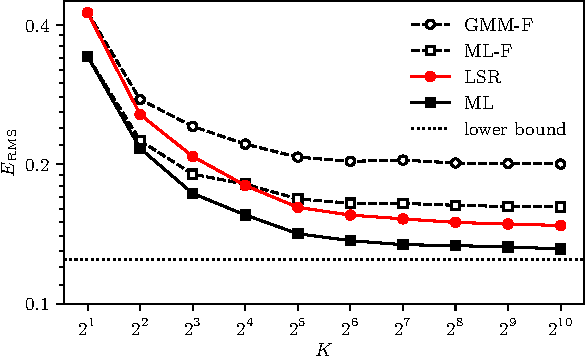
\includegraphics{fi-efficiency}
\caption{
Statistical efficiency of different estimators for increasing sizes of partial rankings.
As $K$ grows, breaking rankings into pairwise comparisons becomes increasingly inefficient.
LSR remains efficient at no additional computational cost.
}
\label{fi:fig:efficiency}
\end{figure}

\subsection{Empirical Performance}

We investigate the performance of various inference algorithms on five real-world datasets.
The NASCAR \citep{hunter2004mm} and sushi \citep{kamishima2009efficient} datasets contain multiway partial rankings.
The YouTube\footnote{%
See: \url{https://archive.ics.uci.edu/ml/machine-learning-databases/00223/}.},
GIFGIF\footnote{%
See: \url{http://lucas.maystre.ch/gifgif-data}.}
and chess datasets\footnote{%
See: \url{https://www.kaggle.com/c/chess}.}
contain pairwise comparisons.
Among those, the chess dataset is particular in that it features 45\% of ties;
in this case we use the extension of the Bradley--Terry model proposed by \citet{rao1967ties}.
We preprocess each dataset by discarding items that are not part of the largest strongly connected component in the comparison graph.
For each dataset, the number of items $N$, the number of rankings $M$, as well as the size $K$ of a partial ranking are given in Table~\ref{fi:tab:approxalg}.
Additional details on the experimental setup are given in the supplementary material.
We first compare the estimates produced by three approximate ML inference algorithms, LSR, GMM-F and Rank Centrality (RC).
Note that RC applies only to pairwise comparisons, and that LSR is the only algorithm able to infer the parameters in the Rao-Kupper model.
Also note that in the case of pairwise comparisons, GMM-F and LSR are strictly equivalent.
In Table~\ref{fi:tab:approxalg}, we report the root-mean-square deviation to the ML estimate $\bm{\theta}^\star$ and the running time $T$ of the algorithm.

\sisetup{group-minimum-digits=4,detect-weight=true}
\begin{table}[ht]
  \caption{Performance of approximate ML inference algorithms}
  \label{fi:tab:approxalg}
  \centering
  \small{
  \begin{tabular}{l rrr rr rr rr rr}
    \toprule
            &             &               &          & \multicolumn{2}{c}{LSR}            & \multicolumn{2}{c}{GMM-F}          & \multicolumn{2}{c}{RC} \\
                                                       \cmidrule(l){5-6}                    \cmidrule(l){7-8}                    \cmidrule(l){9-10}
    Dataset &         $N$ &           $M$ &      $K$ &     $E_{\text{RMS}}$ &     $T$ [s] &     $E_{\text{RMS}}$ &     $T$ [s] & $E_{\text{RMS}}$ & $T$ [s] \\
    \midrule
    NASCAR  &    \num{83} &      \num{36} & \num{43} & \bfseries\num{0.194} &  \num{0.03} &          \num{0.751} &  \num{0.06} &         --- &         --- \\
    Sushi   &   \num{100} &    \num{5000} & \num{10} & \bfseries\num{0.034} &  \num{0.22} &          \num{0.130} &  \num{0.19} &         --- &         --- \\
    \addlinespace                                                                                                             
    YouTube & \num{16187} & \num{1128704} &  \num{2} & \bfseries\num{0.417} & \num{34.18} & \bfseries\num{0.417} & \num{34.18} & \num{0.432} & \num{41.91} \\
    GIFGIF  &  \num{5503} &   \num{95281} &  \num{2} & \bfseries\num{1.286} &  \num{1.90} & \bfseries\num{1.286} &  \num{1.90} & \num{1.295} &  \num{2.84} \\
    \addlinespace                                                                                                             
    Chess   &  \num{6174} &   \num{63421} &  \num{2} & \bfseries\num{0.420} &  \num{2.90} &                  --- &         --- &         --- &         --- \\
    \bottomrule
  \end{tabular}
  }
\end{table}

The smallest value of $E_{\text{RMS}}$ is highlighted in bold for each dataset.
We observe that in the case of multiway partial rankings, LSR is almost four times more accurate than GMM-F on the datasets considered.
In the case of pairwise comparisons, RC is slightly worse than LSR and GMM-F, because the number of comparisons per pair is not homogeneous (see Section~\ref{fi:sec:pairwise}.)
The running time of the three algorithms is comparable.

Next, we turn our attention to ML inference and consider three iterative algorithms: I-LSR, MM and Newton-Raphson.
For Newton-Raphson, we use an off-the-shelf solver.
Each algorithm is initialized with $\bm{\gamma}^{(0)} = [1/N \; \cdots \; 1/N]^\tr$, and convergence is declared when $E_{\text{RMS}} < 0.01$.
In Table~\ref{fi:tab:mlalg}, we report the number of iterations $I$ needed to reach convergence, as well as the total running time $T$ of the algorithm.

\begin{table}[ht]
  \caption{Performance of iterative ML inference algorithms.}
  %The algorithms are stopped when the estimate has a RMSE $< 0.01$.}
  \label{fi:tab:mlalg}
  \centering
  \small{
  \begin{tabular}{l r rr rr rr}
    \toprule
             &             & \multicolumn{2}{c}{I-LSR}        & \multicolumn{2}{c}{MM}      & \multicolumn{2}{c}{Newton} \\
                             \cmidrule(l){3-4}                  \cmidrule(l){5-6}             \cmidrule(l){7-8}
    Dataset  & $\kappa$               & $I$ &         $T$ [s] &        $I$ &        $T$ [s] &     $I$ &     $T$ [s] \\
    \midrule
    NASCAR   & \num{0.832} &  \num{3} &   \bfseries\num{0.08} &    \num{4} &     \num{0.10} &     --- &         --- \\
    Sushi    & \num{0.899} &  \num{2} &   \bfseries\num{0.42} &    \num{4} &     \num{1.09} & \num{3} & \num{10.45} \\
    \addlinespace
    YouTube  & \num{0.002} & \num{12} & \bfseries\num{414.44} & \num{8680} & \num{22443.88} &     --- &         --- \\
    GIFGIF   & \num{0.408} & \num{10} &  \bfseries\num{22.31} &  \num{119} &   \num{109.62} & \num{5} & \num{72.38} \\
    \addlinespace
    Chess    & \num{0.007} & \num{15} &  \bfseries\num{43.69} &  \num{181} &    \num{55.61} & \num{3} & \num{49.37} \\
    \bottomrule
  \end{tabular}
  }
\end{table}

The smallest total running time $T$ is highlighted in bold for each dataset.
We observe that Newton-Raphson does not always converge, despite the log-likelihood being strictly concave\footnote{
On the NASCAR dataset, this has also been noted by \citet{hunter2004mm}.
Computing the Newton step appears to be severely ill-conditioned for many real-world datasets.
We believe that it can be addressed by a careful choice of starting point, step size, or by monitoring the numerical stability;
however, these modifications are non-trivial and impose an additional burden on the practitioner.
}.
I-LSR consistently outperforms MM and Newton-Raphson in running time.
Even if the average running time per iteration is in general larger than that of MM, it needs considerably fewer iterations:
For the YouTube dataset, I-LSR yields an increase in speed of over $50$ times.

The slow convergence of minorization-maximization algorithms is known \cite{hunter2004mm}, yet the scale of the issue and its apparent unpredictability is surprising.
In Hunter's MM algorithm, updating a given $\gamma_i$ involves only parameters of items to which $i$ has been compared.
Therefore, we speculate that the convergence rate of MM is dependent on the expansion properties of the comparison graph $\mathcal{G}$.
As an illustration, we consider the sushi dataset.
To quantify the expansion properties, we look at the spectral gap $\kappa$ of a simple random walk on $\mathcal{G}$;
intuitively, the larger the spectral gap is, the better the expansion properties are \citep{levin2008markov}.
The original comparison graph is almost complete, and $\kappa = 0.899$.
By breaking each \num{10}-way ranking into \num{5} independent pairwise comparisons, we effectively sparsify the comparison graph.
As a result, the spectral gap decreases to \num{0.815}.
In Figure~\ref{fi:fig:convergence}, we show the convergence rate of MM and I-LSR for the original ($K = 10$) and modified ($K = 2$) datasets.
We observe that both algorithms display linear convergence, however the rate at which MM converges appears to be sensitive to the structure of the comparison graph.
In contrast, I-LSR is robust to changes in the structure.
The spectral gap of each dataset is listed in Table~\ref{fi:tab:mlalg}.
%Therefore, to better interpret the result of Table~\ref{fi:tab:mlalg}, we also list for each dataset the spectral gap of its comparison graph.


\begin{figure}[ht]
\centering
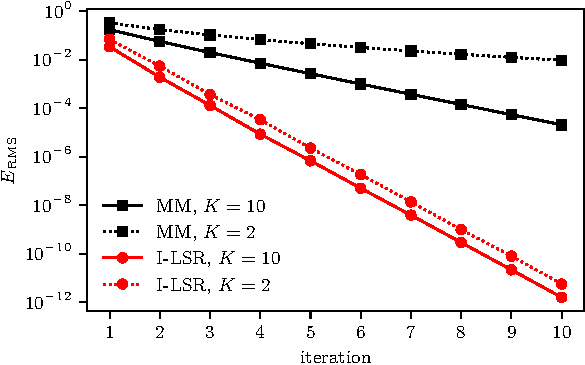
\includegraphics{fi-convergence}
\caption{
Convergence rate of I-LSR and MM on the sushi dataset.
When partial rankings ($K = 10$) are broken down into independent comparisons ($K = 2$), the comparison graph becomes sparser.
I-LSR is robust to this change, whereas the convergence rate of MM significantly decreases.
}
\label{fi:fig:convergence}
\end{figure}

%%%%%%%%%%%%%%%%%%%%%%%%%%%%%%%%
\section{Summary}
\label{fi:sec:summary}

In this chapter, we develop a stationary-distribution perspective on the maximum-likelihood estimate of Luce's choice model.
This perspective explains and unifies several recent spectral algorithms from an ML inference point of view.
We present our own spectral algorithm that works on a wider range of data, and show that the resulting estimate significantly outperforms previous approaches in terms of accuracy.
We also show that this simple algorithm, with a straighforward adaptation, can produce a sequence of estimates that converge to the ML estimate.
On real-world datasets, our ML algorithm is always faster than the state of the art, at times by up to two orders of magnitude.

Beyond statistical and computational performance, we believe that a key strength of our algorithms is that they are simple to implement.
As an example, our implementation of LSR fits in ten lines of Python code.
The most complex operation---finding a stationary distribution---can be readily offloaded to commonly available and highly optimized linear-algebra primitives.
As such, we believe that our work is very useful for practitioners.


%\newcommand{\D}[2]{\ensuremath{\mathcal{D}_{#1 \succ #2}}}

\section{Stationary points of the log-likelihood}

In this section, we briefly explain why the log-likelihood in Luce's model has a unique stationary point, that at the ML estimate.
Recall that we assume that the comparison graph $G_{\mathcal{D}}$ is strongly connected.
The log-likelihood is given by
\begin{align}
\label{eq:loglik}
\log \mathcal{L}(\bm{\pi} \mid \mathcal{D}) = \sum_{\ell = 1}^d \left( \log \pi_\ell - \log{\sum_{j \in A_\ell} \pi_j} \right).
\end{align}
This function is not concave in $\bm{\pi}$; however, this does not preclude the existence of a unique stationary point.
Letting $\pi_i = e^{\theta_i}$, we write the reparametrized log-likelihood as
\begin{align*}
\log \mathcal{L}(\bm{\pi}(\bm{\theta}) \mid \mathcal{D}) = \sum_{\ell = 1}^d \left( \theta_\ell - \log{\sum_{j \in A_\ell} e^{\theta_j}} \right),
\end{align*}
which is strictly concave in $\bm{\theta}$ and therefore admits a unique stationary point, at the maximum of the function.
Denote this maximum by $\hat{\bm{\theta}}$.
The partial derivative of the log-likelihood with respect to $\pi_\ell$ is
\begin{align}
\frac{\partial \log \mathcal{L}}{\partial \pi_\ell}
  = \frac{\partial \log \mathcal{L}}{\partial \theta_i} \cdot \frac{\partial \theta_i}{\partial \pi_i}
  = \frac{\partial \log \mathcal{L}}{\partial \theta_i} \cdot \frac{1}{\pi_i}.
\end{align}
As $1/\pi_i$ is strictly positive, the partial derivative vanishes only at $\hat{\pi}_i = e^{\hat{\theta}_i}$.
In conclusion, $\hat{\bm{\pi}}$ is the unique ML estimate, as well as the only stationary point.


\section{Proofs of Theorems 1 and 2}


For any two items $i$ and $j$, recall that $\mathcal{D}_{i \succ j} \subseteq \mathcal{D}$ is the set of observations where $i$ wins over $j$.
Let $\Delta_n = \{ \bm{u} \in \mathbf{R}^n \mid u_i > 0, \sum_i u_i = 1 \}$ be the open $(n\!-\!1)$-dimensional simplex.
Recall that for $\mathcal{S} \subseteq \mathcal{D}$ and $\vpi \in \Delta_n$, we define
\begin{align}
\label{eq:rate}
f(\mathcal{S}, \bm{\pi}) \doteq \sum_{A \in \mathcal{S}} \frac{1}{\sum_{i \in A} \pi_i}.
\end{align}
We will now prove the following theorem.

\begin{theorem}
\label{thm:convergence}
The Markov chain with inhomogeneous transition rates $\lambda_{ji} = f(\mathcal{D}_{i \succ j}, \vpi)$ converges to the maximum-likelihood estimate $\mlpi$, for any initial distribution $\vpi^0 \in \Delta_n$.
\end{theorem}

We take a discrete-time perspective, and consider the uniformized Markov chain with (parametric) transition probabilities
\begin{align}
  P(\bm{\pi})_{ij} =
  \begin{dcases}
    \epsilon \sum_{A \in \D{j}{i}} \frac{1}{\sum_{t \in A} \pi_t}              & \text{if } j \ne i, \\
    1 - \epsilon \sum_{k \ne i}\sum_{A \in \D{k}{i}} \frac{1}{\sum_{t \in A} \pi_t}  & \text{if } j = i,
  \end{dcases}
\end{align}
where $\epsilon$ (the uniform rate parameter) is a small factor that ensures that the matrix is row-stochastic.
We say that the Markov chain is \emph{inhomogeneous} because the transition probabilities depend on the current distribution over states;
as a consequence, standard ergodic results do not apply directly.
From the development at the beginning of Section 3 of the main text, it follows that $\mlpi$ is the unique invariant distribution of the Markov chain, i.e., satisfying $\mlpi = \mlpi P(\mlpi)$.
Consider the mapping $T: \Delta_n \to \Delta_n$ defined by
\begin{align}
\label{eq:mapping}
T(\vpi) = \vpi P(\vpi),
\end{align}
representing the distribution after one step of the Markov chain.
Using a contraction argument, we will show that the iteration $\vpi^{k+1} = T(\vpi^k)$ converges to a fixed point for any $\vpi^0 \in \Delta_n$.
It directly follows that the Markov chain converges to $\mlpi$ from any initial distribution.

We start with a technical lemma that characterizes the Jacobian matrix of the mapping.
We will use the notation
\begin{align}
T^k(\vpi) = \underbrace{T \circ T \circ \ldots \circ T}_{\text{$k$ times}}(\vpi)
\end{align}
for $k$ successive applications of the mapping.
We will also extend our notation for subsets of observations, and let $\D{i}{j,k} \subseteq \mathcal{D}$ be the observations where $i$ wins among a set of alternatives containing $j$ and $k$.
\begin{lemma}
\label{lem:jacobian}
The Jacobian matrix of the mapping $T(\vpi)$ defined in \eqref{eq:mapping} is given by
\begin{align}
T'(\vpi)_{ij} = \left[ \frac{\partial T(\vpi)}{\partial \pi_i} \right]_j =
\begin{dcases}
\epsilon \sum_{k} \sum_{A \in \D{k}{j,i}} \frac{\pi_j}{(\sum_{t \in A} \pi_t)^2}                          & \text{if } j \ne i, \\
1 - \epsilon \sum_{j \ne \ell} \sum_{k} \sum_{A \in \D{k}{j,\ell}} \frac{\pi_j}{(\sum_{t \in A} \pi_t)^2} & \text{if } j = i.
\end{dcases}
\end{align}
Furthermore, there is a finite $m \in \mathbf{N}$ such that for $S' = (T^m)'$ it holds that $\delta = \min_{i,j} S'_{ij} > 0$ and $\Vert S' \Vert_1 = 1$.
\end{lemma}

\begin{proof}
The partial derivative of $T$ with respect to $\pi_\ell$ at $j \ne \ell$ is
\begin{align}
\left[ \frac{\partial T(\vpi)}{\partial \pi_\ell} \right]_j
&= \left[ \frac{\partial \vpi}{\partial \pi_\ell} P(\vpi) \right]_j + \left[ \vpi \frac{\partial P(\vpi)}{\partial \pi_\ell} \right]_j \\
\begin{split}
&= \epsilon \sum_{A \in \D{j}{\ell}} \frac{1}{\sum_{t \in A} \pi_t}
    - \epsilon \sum_{k \ne j} \sum_{A \in \D{j}{k,\ell}} \frac{\pi_k}{(\sum_{t \in A} \pi_t)^2} \\
    & \qquad\qquad\qquad\qquad\quad + \epsilon \sum_{k \ne j} \sum_{A \in \D{k}{j,\ell}} \frac{\pi_j}{(\sum_{t \in A} \pi_t)^2}
\end{split} \label{eq:before}\\
&= \epsilon \sum_{A \in \D{j}{\ell}} \frac{\pi_j}{(\sum_{t \in A} \pi_t)^2}
    + \epsilon \sum_{k \ne j} \sum_{A \in \D{k}{j,\ell}} \frac{\pi_j}{(\sum_{t \in A} \pi_t)^2} \label{eq:after}\\
&= \epsilon \sum_{k} \sum_{A \in \D{k}{j,\ell}} \frac{\pi_j}{(\sum_{t \in A} \pi_t)^2}.
\end{align} 
To go from \eqref{eq:before} to \eqref{eq:after}, we reverse the order of summation in the subtracted term and rewrite the fraction inside the left term.
\begin{align}
 & \sum_{A \in \D{j}{\ell}} \frac{1}{\sum_{t \in A} \pi_t}
    - \sum_{k \ne j} \sum_{A \in \D{j}{k,\ell}} \frac{\pi_k}{(\sum_{t \in A} \pi_t)^2} \\
=& \sum_{A \in \D{j}{\ell}} \frac{1}{\sum_{t \in A} \pi_t}
    - \sum_{A \in \D{j}{\ell}} \sum_{k \in A, k \ne j} \frac{\pi_k}{(\sum_{t \in A} \pi_t)^2} \\
=& \sum_{A \in \D{j}{\ell}} \sum_{k \in A} \frac{\pi_k}{(\sum_{t \in A} \pi_t)^2}
    - \sum_{A \in \D{j}{\ell}} \sum_{k \in A, k \ne j} \frac{\pi_k}{(\sum_{t \in A} \pi_t)^2} \\
=& \sum_{A \in \D{j}{\ell}} \frac{\pi_j}{(\sum_{t \in A} \pi_t)^2}
\end{align}
One can find the partial derivative with respect to $\pi_\ell$ at $\ell$ by noticing that each row of the Jacobian matrix sums to one:
\begin{align}
\sum_j \left[ \frac{\partial T(\vpi)}{\partial \pi_\ell} \right]_j
&=\sum_j P(\vpi)_{\ell j} + \sum_j \sum_i \pi_i \frac{\partial P(\vpi)_{ij}}{\partial \pi_\ell} \\
&= 1 + \sum_i \pi_i \frac{\partial}{\partial \pi_\ell} \sum_j P(\vpi)_{ij} = 1.
\end{align}
The matrix is therefore row-stochastic, and $\Vert T'(\vpi) \Vert_1 = 1$.
Because transition probabilities are strictly positive on the edges of the comparison graph (which is, by assumption, strongly connected), there is a finite $m \in \mathbf{N}$ such that all entries of $T^m(\vpi)$ are lower-bounded by a strictly positive number.
It is easy to see that the Jacobian matrix $T'$ also has strictly positive entries on the edges of the comparison graph, and therefore
\begin{align}
S'(\vpi) = (T^m(\vpi))' = \prod_{i = 0}^{m-1} T'(T^i(\vpi))
\end{align}
also has its entries lower-bounded by a strictly positive number.
Furthermore, $S'(\vpi)$ is a product of stochastic matrices, hence $\Vert S'(\vpi) \Vert_1 = 1$.
\end{proof}

Now we will use the properties of the Jacobian matrix to show that $T$ is a fixed-point iteration, using a standard argument.
Our proof is inspired by the lecture notes of \citet{tresch2007convergence} and \citet{petersdorff2014fixed}.

\begin{proof}[Proof of Theorem~\ref{thm:convergence}]
Using the results of Lemma~\ref{lem:jacobian}, let $S(\vpi) = T^m(\vpi)$ and write $S'(\vpi)$ as
\begin{align}
S'(\vpi) = \delta 1_{n \times n} + R(\vpi),
\end{align}
where $1_{n \times n}$ is the all-ones matrix, and $\Vert R(\vpi) \Vert_1 = 1 - n\delta = c < 1$.
Now pick any $\bm{x}, \bm{y} \in \Delta_n$, and let $\tilde{S}(u) \doteq S(\bm{x} + u(\bm{x} - \bm{y}))$.
Then $\tilde{S}'(u) = S'(\bm{x} + u(\bm{y} - \bm{x}))(\bm{y} - \bm{x})$, and
\begin{align}
S(\bm{y}) - S(\bm{x}) = \tilde{S}(1) - \tilde{S}(0) = \int_0^1 \tilde{S}'(u) du = \int_0^1 S'(\bm{x} + u(\bm{y} - \bm{x}))(\bm{y} - \bm{x}) du
\end{align}
As $S'$ is continuous, we have
\begin{align}
\Vert S(\bm{y}) - S(\bm{x}) \Vert_1 &\le \int_0^1 \Vert S'(\bm{x} + u(\bm{y} - \bm{x}))(\bm{y} - \bm{x}) \Vert_1 du \\
&=   \int_0^1 \Vert \underbrace{\delta 1_{n \times n}(\bm{y} - \bm{x})}_{= 0} + R(\bm{x} + u(\bm{y} - \bm{x}))(\bm{y} - \bm{x}) \Vert_1 du \\
&\le \int_0^1 \underbrace{\Vert R(\bm{x} + u(\bm{y} - \bm{x})) \Vert_2}_{\le c} \Vert \bm{y} - \bm{x} \Vert_1 du \\
&\le c \Vert \bm{y} - \bm{x} \Vert_1
\end{align}
Therefore, by the contraction mapping principle, the sequence of iterates $\vpi^{k+1} = T^m(\vpi^k)$ converges to $\mlpi$.
Finally, we observe that for any $\vpi \in \Delta_n$, the vectors $\vpi, T(\vpi), T^2(\vpi), \ldots$ occur in one of the sequences
\begin{align}
\left( S^k(T^r(\vpi)) \right)_{k \in \mathbf{N}_0}, \quad r \in \{ 0, \ldots, m\!-\!1 \}.
\end{align}
All sequences converge to $\mlpi$, and therefore
\begin{align}
\lim_{k \to \infty} T^k(\vpi) = \mlpi.
\end{align}
\end{proof}

\begin{theorem}
\label{thm:consistency}
Let $\mathcal{A} = \{ A_\ell \}$ be a collection of sets of alternatives such that for any partition of $\mathcal{A}$ into two non-empty sets $S$ and $T$, $\left( \cup_{A \in S} A \right) \cap \left( \cup_{A \in T} A \right) \ne \varnothing$.
Let $d_\ell$ be the number of choices observed over alternatives $A_\ell$.
Then $\rcpi \to \bm{\pi}^*$ as $d_\ell \to \infty \ \forall \ell$.
\end{theorem}

\begin{proof}
Let $d \to \infty$ be a shorthand for $d_\ell \to \infty \ \forall \ell$.
The condition on $\mathcal{A}$ is equivalent to stating that the hypergraph $H = (V, \mathcal{A})$ with $V = \{1, \ldots, n\}$ is connected.
First, we show that asymptotically, the graph $G_\mathcal{D} = (V, E)$ is connected.
For a given set of alternatives $A_\ell$, let $i, j \in A_\ell$.
The probability that $(j, i) \in E$ is
\begin{align}
1 - \left(1 - \frac{\pi_i}{\sum_{t \in A_\ell} \pi_t} \right)^{d_\ell}
> 1 - (1 - \pi_i)^{d_\ell}
\xrightarrow{d_\ell \to \infty} 1,
\end{align}
where we use the fact that $\pi_i > 0 \ \forall i$.
Therefore, asymptotically, every alternative set $A_\ell$ forms a clique in $G_\mathcal{D}$.
By assumption of connectivity on the hypergraph $H$, $G_{\mathcal{D}}$ is strongly connected.

Now that we know that the Markov chain is asymptotically ergodic, we will show that the stationary distribution matches the true model parameters.
Let $C_\ell^s$ be a random variable denoting the item chosen in the $s$-th observation over alternatives $A_\ell$.
By the law of large numbers, for any item $i \in A_\ell$
\begin{align}
\label{eq:lln}
\lim_{d_\ell \to \infty} \frac{1}{d_\ell} \sum_{s = 1}^{d_\ell} 1\{C_\ell^s = i\} = \frac{\pi^*_i}{\sum_{t \in A_\ell} \pi^*_t}.
\end{align}
Now consider two items $i$ and $j$.
If they have never been compared, $\lambda_{ij} = \lambda_{ji} = 0$.
Otherwise, suppose that they have been compared in alternative sets whose indices are in $B = \{ \ell \mid i, j \in A_\ell \}$
Let $\mathbf{1}\{X\}$ be the indicator variable for event $X$.
By construction of the transition rates in \LSR{}, we have that
\begin{align}
\label{eq:ratio}
\frac{\lambda_{ij}}{\lambda_{ji}}
= \frac{\sum_{\ell \in B} \sum_{s = 1}^{d_\ell} \mathbf{1}\{C_\ell^s = j\} \ n / |A_\ell|}
       {\sum_{\ell \in B} \sum_{s = 1}^{d_\ell} \mathbf{1}\{C_\ell^s = i\} \ n / |A_\ell|}.
\end{align}
From \eqref{eq:lln} it follows that
\begin{align}
\lim_{d \to \infty}\frac{\lambda_{ij}}{\lambda_{ji}}
& = \frac{\sum_{\ell \in B} (\pi^*_j / \sum_{t \in A_\ell} \pi^*_t) \ n / |A_\ell|}
         {\sum_{\ell \in B} (\pi^*_i / \sum_{t \in A_\ell} \pi^*_t) \ n / |A_\ell|} \\
& = \frac{\pi^*_j }{\pi^*_i}
    \cdot \frac{\sum_{\ell \in B}(1 / \sum_{t \in A_\ell} \pi^*_t) \ n / |A_\ell|}
               {\sum_{\ell \in B}(1 / \sum_{t \in A_\ell} \pi^*_t) \ n / |A_\ell|}
  = \frac{\pi^*_j}{\pi^*_i}.
\end{align}
Therefore, when $d \to \infty$,
\begin{align}
\sum_{j \ne i} \pi^*_i \lambda_{ij} = \sum_{j \ne i} \pi^*_i \left( \frac{\pi^*_j}{\pi^*_i} \lambda_{ji} \right)
                                    = \sum_{j \ne i} \pi^*_j \lambda_{ji}  \quad \forall i.
\end{align}
It is easy to recognize the global balance equations, and it follows that $\bm{\pi}^*$ is the stationary distribution of the asymptotical Markov chain.
\end{proof}


\section{Bound on error rate of ML estimate}

We use the analytical framework of \citet{negahban2017rank} to bound the error rate of the ML estimator in the case where
\begin{enuminline}
\item the data is in the form of pairwise comparisons and
\item for each pair under comparison, we observe exactly $k$ outcomes.
\end{enuminline}

Let $G = (V, E)$ be an undirected graph where $V = \{ 1, \ldots, n \}$ and $(i, j) \in E$ if $i$ and $j$ have been compared.
Let $d_{\min}$ and $d_{\max}$ be the minimum and maximum degree of a node in $G$, respectively.
Let $\gamma$ be the spectral gap of a simple random walk on $G$;
intuitively, the larger the spectral gap is, the faster the convergence to the stationary distribution is.
For each $(i, j) \in E$ we observe $k$ comparisons generated from ground truth parameters $\bm{\pi}^*$.
Let $A_{ji}$ denote the number of times $i$ wins against $j$ and $a_{ji} = A_{ji} / k$ the ratio of wins of $i$ over $j$.
We say that an event $X$ occurs with high probability if $\mathbf{P}(X) \ge 1 - c / n^\alpha$ for $c, \alpha$ fixed.

\begin{theorem}
\label{thm:mlbound}
For $k \ge 4C^2 (1 + (b^6 \kappa^2 / (d_{\max} \gamma^2)) \log n)$, the error on the ML estimate $\mlpi$ satisfies w.h.p.
\begin{align}
\frac{\Vert \mlpi - \bm{\pi}^* \Vert_2}{\Vert \bm{\pi}^* \Vert_2} < C \frac{b^{7/2} \kappa}{\gamma} \sqrt{\frac{\log n}{kd_{\max}}},
\end{align}
where $C$ is a constant, $b = \max_{i,j} \pi^*_i / \pi^*_j$ and $\kappa = d_{\max} / d_{\min}$.
\end{theorem}

\begin{proof}
The ML estimate can be interpreted as the stationary distribution of the discrete-time Markov chain
\begin{align}
\label{eq:mlchain}
  \widehat{P}_{ij} =
  \begin{dcases}
    \epsilon \frac{a_{ij}}{\hat{\pi}_i + \hat{\pi}_j}                    & \text{if } i \ne j, \\
    1 - \epsilon \sum_{l \ne i} \frac{a_{il}}{\hat{\pi}_i + \hat{\pi}_l} & \text{if } i = j.
  \end{dcases}
\end{align}
The factor $\epsilon = \hat{\pi}_{\min} / d_{\max}$ ensures that $\widehat{P}$ is stochastic.
Given this matrix, it is straightforward to analyze the $\mlpi$ by using the methods developed for Rank Centrality (RC);
the proof essentially follows that of Theorem~1 of \citet{negahban2017rank}.
Let $P^*$ be the ideal Markov chain, when  $a_{ij} = \pi^*_j / (\pi^*_i + \pi^*_j)$, i.e., the ratios are noiseless.
The key observation is to note that the stationary distribution of $P^*$ is $\bm{\pi}^*$, the true model parameters.
By bounding $\Vert \widehat{P} - P^* \Vert_2$ and $1 - \lambda_{\max}(P^*)$, we can bound the error on the stationary distribution of $P^*$.
For the former, a straightforward application of the proof in the RC case suffices.
For the latter, in the application of the comparison theorem, the lower bound on $\min_{i,j} \pi^*_i P^*_{ij}$ changes by a factor of $1/(2b)$.
This is due to the additional factor $\hat{\pi}_{\min} / (\hat{\pi}_i + \hat{\pi}_j)$ in the off-diagonal entries of $P^*$.
\end{proof}

If the graph of comparisons $G$ is an expander, then $\gamma = O(1)$.
Furthermore, if $d_{\max} \propto d_{\min}$, then $\kappa = O(1)$.
A realization of the $G(n, p)$ random graph satisfies these two constraints with high probability as long as $p = \omega(\log n / n)$.
It follows that if $\omega(n \log n)$ comparison pairs are chosen uniformly at random and $k = O(1)$ outcomes are observed for each pair, the error goes to zero as $n$ increases.

\citet{hajek2014minimax} recently proved a more general version of our result, using a different analytical technique.
Their bound is qualitatively similar, but also applies to multiway rankings and heterogeneous number of comparisons.

\section{Derivation for the Rao--Kupper model}

We consider a model that was proposed by Rao and Kupper in 1967 \citep{rao1967ties}.
This model extends the Bradley--Terry model in that a comparison between two items can result in a tie.
Letting $\alpha \in [1, \infty)$, the probabilities of $i$ winning over and tying with $j$, respectively, are given as follows.
\begin{align*}
p(i \succ j) &= \frac{\pi_i}{\pi_i + \alpha \pi_j}, \\
p(i \leftrightarrow j) &= \frac{\pi_i \pi_j(\alpha^2 - 1)}{(\pi_i + \alpha\pi_j)(\alpha \pi_i + \pi_j)}.
\end{align*}
This model is useful for e.g., chess, where a significant fraction of comparison outcomes do not result in either a win or a loss.

We assume that the parameter $\alpha$ is fixed, and derive an expression of the ML estimate $\mlpi$.
Let $A_{ji}$ be the number of times $i$ wins over $j$, and $T_{ij} = T_{ji}$ be the number of ties between $i$ and $j$.
The log-likelihood can be written as
\begin{align}
\log \mathcal{L} &=
  \sum_i \sum_{j \ne i}
  A_{ji} \left( \log(\pi_i) - \log(\pi_i + \alpha \pi_j) \right) \\
    &+ \sum_i \sum_{j > i} \nonumber
    T_{ij} ( \log(\pi_i) + \log(\pi_j) + \log(\alpha^2 - 1) \\
    & \qquad \qquad {} - \log(\pi_i + \alpha \pi_j) - \log(\alpha \pi_i + \pi_j) ). \nonumber
\end{align}
The log-likelihood function is strictly concave and the model admits a unique ML estimate $\mlpi$.
The optimality condition $\nabla_{\mlpi} \log \mathcal{L} = 0$ implies
\begin{align}
  \frac{\partial \log \mathcal{L}}{\partial \hat{\pi}_i}
  = &\sum_{j \ne i} A_{ji} \left( \frac{1}{\hat{\pi}_i} - \frac{1}{\hat{\pi}_i + \alpha \hat{\pi}_j} \right)
    - A_{ij} \frac{\alpha}{\alpha \hat{\pi}_i + \hat{\pi}_j} \\
  & \qquad {} + T_{ij} \left( \frac{1}{\hat{\pi}_i} - \frac{1}{\hat{\pi}_i + \alpha \hat{\pi}_j} - \frac{\alpha}{\alpha \hat{\pi}_i + \hat{\pi}_j}\right) = 0 \\
  \iff & \sum_{j \ne i} A_{ji} \frac{\alpha \hat{\pi}_j}{\hat{\pi}_i + \alpha \hat{\pi}_j}
    - A_{ij} \frac{\alpha \hat{\pi}_i}{\alpha \hat{\pi}_i + \hat{\pi}_j} \\
  & \qquad {} + T_{ij} \frac{\alpha \hat{\pi}_j^2 - \alpha \hat{\pi}_i^2}{(\hat{\pi}_i + \alpha \hat{\pi}_j)(\alpha \hat{\pi}_i + \hat{\pi}_j)} = 0 \\
  \iff & \sum_{j \ne i} \frac{A_{ji} + T_{ji}\tfrac{\hat{\pi}_j}{\alpha \hat{\pi}_i + \hat{\pi}_j}}{\hat{\pi}_i + \alpha \hat{\pi}_j} \hat{\pi}_j
    - \frac{A_{ij} + T_{ij}\tfrac{\hat{\pi}_i}{\hat{\pi}_i + \alpha \hat{\pi}_j}}{\alpha \hat{\pi}_i + \hat{\pi}_j} \hat{\pi}_i = 0.
\end{align}
Therefore, the ML estimate is the stationary distribution of a Markov chain with transition rates
\begin{align}
\lambda_{ij} = \frac{A_{ij} + T_{ij}\tfrac{\hat{\pi}_i}{\hat{\pi}_i + \alpha \hat{\pi}_j}}{\alpha \hat{\pi}_i + \hat{\pi}_j}.
\end{align}
The extension of \LSR{} and \ILSR{} to the Rao--Kupper model given these transition rates is straightforward.



\section{Finding the stationary distribution}

A set of transition rates $[\lambda_{ij}]$ that satisfy the strong connectivity assumption yields a unique stationary distribution $\bm{\pi}$.
In practice, finding this stationary distribution can be implemented in various ways.
We distinguish implementations based on whether they consider a continuous-time or a discrete-time perspective on Markov chains.

\paragraph{Continuous-time perspective.}
We consider the infinitesimal generator matrix $Q$, where $Q_{ij} \doteq \lambda_{ij}$ and $Q_{ii} \doteq - \sum_{j} \lambda_{ij}$.
The stationary distribution satisfies $\bm{\pi} Q = 0$; this is essentially a matrix formulation of the global balance equations.
Therefore, one approach to finding the steady-state distribution is to compute the rank-$1$ left nullspace of $Q$.
This can be done e.g., by LU decomposition, a basic linear-algebra primitive.
In the dense case, the running time of a typical implementation is $O(n^3)$, but highly optimized parallel implementations such as that provided by LAPACK \citep{anderson1999lapack} are commonly available.
In the sparse case, LU decomposition can be done significantly faster using adapted algorithms, such as that of \citet{demmel1999supernodal}.

\paragraph{Discrete-time perspective.}
Let $\epsilon < 1 / \max_i |Q_{ii}|$, then $P = I + \epsilon Q$ is the transition matrix of a discrete-time Markov chain that satisfies $\bm{\pi} P = \bm{\pi}$.
In this case, finding the steady-state distribution is equivalent to finding the left eigenvector associated to the leading eigenvalue of the transition matrix $P$.
This is also a well-studied linear algebra problem for which plenty of efficient, off-the-shelf algorithms exist.
For example, power iteration methods can find the eigenvector in a few (sparse) matrix multiplications.
Beyond these well-known algorithms, the recently proposed randomized approach of \citet{halko2011finding} enables us to scale to truly large problem sizes ($n$ is $O(10^6)$ or more.)

For our experiments, we have implemented \LSR{} and \ILSR{} using a dense LU factorization of the generator matrix.
The Python code, which relies on the \texttt{numpy} and \texttt{scipy} libraries\footnote{
See: \url{http://www.scipy.org/}.
}, is displayed in Figure~\ref{lst:implementation}

%\lstset{
%  language=Python,
%  basicstyle=\ttfamily\footnotesize,         % Teletype font.
%  showstringspaces=false,       % Don't put underscores in place of spaces.
%  numberstyle=\ttfamily, % Numbers in gray (+ teletype font).
%  numbers=left,                 % Show line numbers on the left.
%  numbersep=5pt,                % Give some space to those poor line numbers.
%  xleftmargin=15pt,             % But don't put them in the margin either.
%  %columns=fixed,               % No idea what this is for.
%}
\begin{figure}
\label{lst:implementation}
\begin{lstlisting}
import numpy as np
import scipy.linalg as spl

def weighted_lsr(n, rankings, weights):
    chain = np.zeros((n, n), dtype=float)
    for ranking in rankings:
        sum_weights = sum(weights[x] for x in ranking)
        for i, winner in enumerate(ranking):
            val = 1.0 / sum_weights
            for loser in ranking[i+1:]:
                chain[loser, winner] += val
            sum_weights -= weights[winner]
    chain -= np.diag(chain.sum(axis=1))
    return statdist(chain)

def statdist(chain):
    lu, piv = spl.lu_factor(generator.T)
    res = spl.solve_triangular(lu[:-1,:-1], -lu[:-1,-1])
    res = np.append(res, 1.0)
    return res / res.sum()
\end{lstlisting}
\caption{
Python implementation of one iteration of \ILSR{}.
}
\end{figure}

\section{Experimental procedure}

We give a few additional details on the procedure that we followed for the experiments of Section~4 in the main paper.
All experiments were run on a machine with a quad-core 2.0 GHz Haswell processor, and 16GB of RAM, running Mac OS X 10.9.
For \LSR{} and \ILSR{}, we used a slightly adapted version the code presented in Figure~\ref{lst:implementation}.
We implemented the Rank Centrality (RC), GMM-F \citep{azari2013generalized}, and MM \citep{hunter2004mm} algorithms in Python.
For Newton-Raphson, we implemented our choice model on top of the popular \texttt{statsmodels} Python library\footnote{
See: \url{http://statsmodels.sourceforge.net/}
} that provides a Newton-Raphson solver.
For completeness, the Python source code containing all the functions we used is provided as a separate file in the supplementary material.
We have compared our implementation of the MM algorithm to that of \citeauthor{hunter2004mm} written in Matlab\footnote{
See: \url{http://sites.stat.psu.edu/~dhunter/code/btmatlab/}
}, and observed that ours has comparable running time.

For the chess dataset, we use the Rao--Kupper model and set the parameter $\alpha = \sqrt{2}$.
Note that this parameter could also be estimated from the data, however in our experiments we focus on the performance of algorithms for estimating $\mlpi$.

